\documentclass[a4paper,11pt]{article}


\usepackage{geometry}
\usepackage[utf8]{inputenc}
\usepackage[francais]{babel}
\usepackage[T1]{fontenc}
\usepackage{tikz-uml}
\usepackage{color}
\definecolor{dkgreen}{rgb}{0,0.6,0}
\definecolor{gray}{rgb}{0.5,0.5,0.5}
\definecolor{mauve}{rgb}{0.58,0,0.82}

\usepackage{listings}
\usepackage{float}
\usepackage{kpfonts}

\usepackage{graphicx}
%% \newcommand{\foofoo}{\hspace{-2.3pt}$\bullet$ \hspace{5pt}}

\lstset{
language=C++,
basicstyle=\footnotesize,
backgroundcolor=\color{white},
keywordstyle=\color{red},
commentstyle=\color{dkgreen},
stringstyle=\color{mauve},
numberstyle=\color{red},
morekeywords={string},
frame=BL,
aboveskip=1em,
belowskip=2em,
}
\lstset{
  literate={ù}{{\`u}}1
           {é}{{\'e}}1
           {è}{{\'e}}1
           {à}{{\`a}}1
}


\lstdefinelanguage{tikzuml}{language=[LaTeX]TeX, classoffset=0, morekeywords={umlbasiccomponent, umlprovidedinterface, umlrequiredinterface, umldelegateconnector, umlassemblyconnector, umlVHVassemblyconnector, umlHVHassemblyconnector, umlnote, umlusecase, umlactor, umlinherit, umlassoc, umlVHextend, umlinclude, umlstateinitial, umlbasicstate, umltrans, umlstatefinal, umlVHtrans, umlHVtrans, umldatabase, umlmulti, umlobject, umlfpart, umlcreatecall, umlclass, umlvirt, umlunicompo, umlimport, umlaggreg}, classoffset=1, morekeywords={umlcomponent, umlsystem, umlstate, umlseqdiag, umlcall, umlcallself, umlfragment, umlpackage}, classoffset=0,  sensitive=true, morecomment=[l]{\%}}

\geometry{margin=2cm}
\geometry{headheight=15pt}

\usepackage{fancyhdr}
\usepackage{fancyvrb}
\usepackage{float}
\usepackage{acronym}
\pagestyle{fancy}
\rhead{PFA - GuitarTutor}

\acrodef{LABRI}{Laboratoire Bordelais de Recherche en Informatique}

\begin{document}

\begin{titlepage}
  \begin{center}

    \textsc{\LARGE PFA - GuitarTutor}\\[2cm]
    Pacien \textsc{Boisson} \ \ \ Jean-Michaël \textsc{Celerier}  \ \ \ Julien \textsc{Chaumont}\\
    Abdelhamid \textsc{Cherif} \ \ \ Alban \textsc{De Martin} \ \ \ Kun \textsc{Jiao} \ \ \ Bastien \textsc{Meunier} \\[3cm]
    \textsc{\large 29/03/2013 }\\[1.5cm]
    
\includegraphics[width=8cm]{logo.png}

  \end{center}
  \vspace{3cm}
  \begin{flushleft}
   \underline{Clients :} Pierre \textsc{Hanna}, Matthias \textsc{Robine}\\
   \underline{Responsable pédagogique :} Julien \textsc{Allali}
  \end{flushleft}


\end{titlepage}

\section*{Introduction}
%Dans cette partie, j'ai repris quasiment mot pour mot l'intro que j'avais écrite pour le cahier des charges.

\subsection*{Serious game}

En quelques années, les jeux vidéos ont su attirer un public immense et éclectique. Alors qu'ils étaient réservés, il y a encore quelques années, à un public bien ciblé, les éditeurs ont su s'ouvrir à toute une gamme de joueurs jusqu'alors insoupçonnés - l'appellation casual gamer était née. Aujourd'hui, les recherches dans le domaine vidéo-ludique vont encore plus loin. A l'aide de technologies toujours plus poussées, toujours plus proches du joueur et de son environnement, il est désormais possible d'interagir avec lui, grâce à ses mouvements par exemple. Et pourquoi pas par le son? Les jeux de rythme, remontant pourtant aux bornes d'arcade des années 1990, ont connu un immense succès avec la sortie de jeux tels que Guitar Hero en 2005, qui a ouvert la voie à de nombreux remakes que sont Just Dance ou encore Band Hero. En parallèle, les jeux à caractère éducatif, ont été pendant longtemps recalés au rang de “sous-jeux” de par leurs gameplays souvent repoussants et des graphismes généralement peu soignés -
évidemment, les budgets ne sont pas forcément les mêmes.

Le projet GuitarTutor se place au croisement de ces deux genres pour s'inscrire dans celui très fermé des serious games: pourquoi ne pas apprendre en s'amusant? (En l'occurrence l'apprentissage de la guitare). Ce jeu s'adresse à des élèves d'écoles de musique débutant la pratique de l'instrument. L'objectif est de les encourager à jouer et à s'entraîner en dehors des heures de cours avec leurs professeurs, en faisant intervenir cet univers ludique, pour les inciter à persévérer et à travailler d'eux-mêmes.

\subsection*{Le logiciel avant le PFA}

Le logiciel GuitarTutor reposait sur des travaux de recherches du \ac{LABRI}, ainsi que sur le travail fourni par des élèves de l'ENSEIRB-MATMECA dans le cadre des Projets au Fil de l'Année (PFA) de 2011-2012. La base du projet consistait en l'analyse d'accords en temps réel, c'est-à-dire pouvoir donner précisément le nom de l'accord qui est donné en entrée audio de l'ordinateur. La librairie EHPCP a donc été codée à cet effet. En complément, le développement d'une interface graphique, à l'aide de la librairie Qt, a été réalisée. Celle-ci assurait le fonctionnement basique d'un logiciel permettant de visualiser une liste défilante d'accords ainsi que le résultat de la partie analyse de l'entrée audio, en comparant cette donnée au résultat attendu.

Afin de faciliter l'écriture des fichiers partitions, un second logiciel avait été mis en place à destination du professeur. Il permettait une édition totalement manuelle de grilles d'accords, ainsi qu'une édition assistée. Ce second mode d'édition demandait à l'utilisateur de marquer les accords d'un morceau joué simultanément par l'appui sur une touche de son clavier. Dans un deuxième temps, il suffisait d'indiquer quels étaient les accords qui correspondaient à chaque pulsation.

\subsection*{Notre objectif}

L'objectif de notre projet était donc de rendre le logiciel existant accessible. Son interface d'origine avait, en effet, plus la carrure d'un prototype que celle d'un produit fini. Un soin particulier devait être apporté à l'éditeur de partitions afin d'optimiser au mieux l'expérience utilisateur. Selon les demandes clients, GuitarTutor devait être un logiciel fini et livrable pour avril 2013.


\tableofcontents

\section{Architecture logicielle}

Nous présenterons dans cette partie la structure du projet actuel, ainsi que celle de sa version d'origine.

\subsection{Architecture du projet d'origine}

Il nous a fallu un certain temps pour comprendre comment était pensé le projet d'origine. Principalement, il y avait une séparation complète entre le lecteur et l'éditeur, et aucune bibliothèque partagée entre les deux.

L'éditeur était divisé en deux sous-programmes : un qui faisait de la lecture audio, et un qui permettait de rentrer des accords dans un
tableau. Le lecteur, quant à lui, était aussi divisé en deux sous-programmes : un qui permettait de lire les donnés de l'éditeur (ce n'était pas fonctionnel),
et un qui permettait de produire un nouveau fichier de données à partir d'un enregistrement de guitare.

Une librairie imposante était fournie ave le lecteur : IScoreLight, une version simplifiée d'un séquenceur complet développé au \ac{LABRI}.

Le problème principal était le fait que le lecteur et l'éditeur n'étaient pas capables d'échanger leurs données. Le fonctionnement multi-plateformes n'était lui non plus pas assuré.

\subsection{Le modèle \ac{MVC}}

Le modèle \ac{MVC}, pour \textit{Modèle, Vue, Contrôleur}, constitue une architecture logicielle particulière qui se base sur la différenciation de deux parties dans un programme:
\begin{itemize}
 \item Les données (le modèle)
 \item L'interface graphique (la vue)
\end{itemize}

Le contrôleur se place entre ces deux entités, en agissant comme relais en synchronisant les informations qui transitent de l'une à l'autre.

L'avantage immédiat du modèle \ac{MVC} est l'organisation du code qu'il induit, ainsi que la facilitation de la maintenance de celui-ci.

\subsubsection{Editeur, Lecteur et \ac{API}}

Il nous a été conseillé dès le début du projet d'adopter le modèle \ac{MVC}. En plus des avantages cités précédemment, cela nous permettait de découvrir le code existant, de mieux le comprendre, et de commencer à le réorganiser correctement. L'architecture qui a été retenue était de découper le projet en trois parties:
\begin{itemize}
 \item L'interface graphique du lecteur
 \item L'interface graphique de l'éditeur
 \item Le reste: l'\ac{API}
\end{itemize}
L'idée était de mettre ce \textit{reste} dans une bibliothèque qui serait appelée à la fois par l'éditeur et par le lecteur (même si ce ne sont pas forcément les mêmes parties qui les intéressent). La figure \ref{mvc} résume cette organisation.

\begin{figure}[H]
\begin{center}
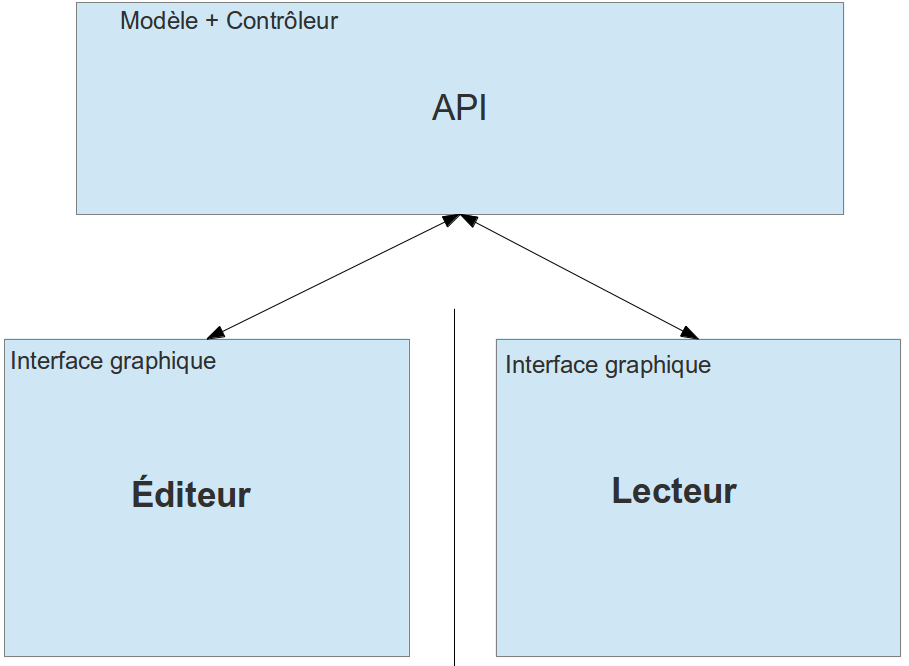
\includegraphics[width=300px]{mvc.png}
\caption{Le modèle MVC dans notre code}
\label{mvc}
\end{center}
\end{figure}


A un autre niveau, nous avons, lorsque c'était facilement appliquable, utilisé le paradigme \ac{MVC} de Qt, ce qui est facilité
par l'utilisation de QtCreator, l'IDE fourni avec Qt. En effet, ce dernier permet de concevoir l'interface graphique directement, et de générer automatiquement le code qui y correspond sans que l'on ait à y toucher, ce qui nous permet de nous concentrer uniquement sur la logique sous-jacente.

On peut notamment s'en rendre compte dans les classes \texttt{TrackProperties} ou \texttt{PartSetter} de l'éditeur.
\subsubsection{L'\ac{API}}

L'\ac{API} a été mise en place dès le début du projet, en regroupant dans un même dossier tous les fichiers sources qui ne concernaient pas directement l'interface graphique du lecteur, ni celle de l'éditeur.

\subsubsection*{La modélisation des accords}

Nous avons ensuite ajouté de nouvelles classes pour modéliser les accords de manière la plus abstraite possible, afin de respecter au mieux les objets Modèle du \ac{MVC}. Nous avons pour cela utilisé trois classes (Tonality, Enrichment, Chord), ainsi que deux énumérations (Note et Alteration) pour définir un accord selon le schéma suivant:
\begin{itemize}
 \item Une \textcolor{blue}{tonalité}, c'est une \textcolor{red}{note} et une \textcolor{green}{altération}: \textcolor{red}{A}\textcolor{green}{$\sharp$}, \textcolor{red}{C}\textcolor{green}{$\flat$}, \textcolor{red}{G}\textcolor{green}{$\natural$}, \dots
 \item Un accord, c'est une \textcolor{blue}{tonalité} et un \textcolor{magenta}{mode}: \textcolor{blue}{G$\flat$}\textcolor{magenta}{m}, \textcolor{blue}{B$\sharp$}\textcolor{magenta}{M}, \dots
\end{itemize}

Cette découpe des modèles se répercute dans l'architecture de ces classes (voir le diagramme de classes de la figure \ref{diag_api_chords}). Bien sûr, différentes méthodes ont été implémentées pour chacune de ces classes, bien qu'en réalité peu d'entre elles soient réellement utilisées par GuitarTutor. C'était néanmoins un bon moyen de repartir sur de bonnes bases au début du projet, et certaines de ces méthodes nous ont finalement été utiles plus tard dans la phase de développement. C'est pourquoi nous avons décidé de les laisser dans l'\ac{API}, dans le cas probable qu'elles soient utiles plus tard à GuitarTutor.

\begin{figure}[H]
\begin{center}
\begin{tikzpicture}
\umlclass[x=-7, y=0]{Chord}{
}{}
\umlclass[x=-13, y=-3]{Enrichment}{
}{}
\umlclass[x=-1, y=-3]{Tonality}{
}{}
\umlclass[x=-1, y=-6]{Note}{
}{}
\umlclass[x=-7, y=-6]{Alteration}{
}{}

\umlunicompo[]{Chord}{Enrichment}
\umlunicompo[]{Chord}{Tonality}
\umlunicompo[]{Tonality}{Alteration}
\umlunicompo[]{Tonality}{Note}
\end{tikzpicture}
\caption{La modélisation des accords dans l'\ac{API}}
\label{diag_api_chords}
\end{center}
\end{figure}

\subsubsection*{La classe \textit{LogicalTrack} et les classes associées}

Ultérieurement, c'est la classe \textit{LogicalTrack} que nous avons mise en place. Cet objet représente en mémoire une grille d'accords. Elle est utilisée par l'éditeur, qui transforme les données entrées par l'utiliseur en une instance de \textit{LogicalTrack}, puis fais la conversion en un fichier XML; et de l'autre côté, elle est utilisée par le lecteur qui initialise un objet \textit{LogicalTrack} à partir de la lecture d'un fichier XML. Sa structure est relativement simple et correspond parfaitement à celle que nous avons choisie d'adopter pour les fichiers XML de sauvegarde de grilles (le format est expliqué plus en détail dans la partie \ref{xml}):
\begin{itemize}
 \item Une grille est une suite de parties (intro, refrain, couplet 1,\dots).
 \item Chaque partie est composée d'une suite de notes
 \item A chaque note correspond un temps de début, le temps de fin étant le début de la note suivante
\end{itemize}

Là encore, le découpage des classes découle parfaitement de cette vision d'une grille (figure \ref{diag_api_tracks}). Parallèlement, la classe \textit{TrackLoader}, elle aussi dans l'\ac{API}, contient deux méthodes statiques qui permettent la conversion d'une instance de \textit{LogicalTrack} vers un fichier XML, ou inversement.

\begin{figure}[H]
\begin{center}
\begin{tikzpicture}
\umlclass[x=-13, y=0]{LogicalTrack}{
}{}
\umlclass[x=-7, y=0]{PartTrack}{
}{}
\umlclass[x=-1, y=0]{TrackChord}{
}{}

\umlunicompo[]{LogicalTrack}{PartTrack}
\umlunicompo[]{PartTrack}{TrackChord}
\end{tikzpicture}
\caption{Modélisation d'une grille d'accords dans l'\ac{API}}
\label{diag_api_tracks}
\end{center}
\end{figure}

\subsubsection*{Les autres rôles de l'\ac{API}}

Comme évoqué en introduction de cette partie, l'\ac{API} a été à la base construite sur les parties du code d'origine n'étant pas directement liées à l'interface. C'est en suivant ce principe que nous avons ajouté à l'\ac{API} la bibliothèque IScoreLight, qui servait à la lecture de grilles d'accord, ainsi que EHPCP qui est utilisée pour la reconnaissance des accords. Dans la même veine, on peut évoquer les classes qui servaient déjà à la gestion audio du lecteur, telles que \textit{Track} (que nous avons plus tard adaptée à nos besoins) pour charger en mémoire un fichier audio, ou \textit{MusicManager}, classe pilier concernant la gestion des entrées et des sorties audio.

\subsubsection{L'éditeur}

Le rôle de l'éditeur est d'assister l'utilisateur pour construire une grille d'accords qui soit lisible et jouable sur le lecteur. En accord avec la conception \ac{MVC}, l'éditeur en lui-même ne regroupe que les éléments se rapportant à l'interface graphique ou ayant des rôles de contrôleurs. La souche de l'éditeur est en fait le widget \textit{GridEditor}, qui sert à la fois d'interface et d'orchestrateur entre les différentes sous-composantes de l'éditeur, à savoir:
\begin{itemize}
 \item \textit{ChordTableWidget}, qui apparaît à l'écran comme un tableau où chaque case (instances de la classe \textit{CaseItem}) doivent contenir un accord
 \item \textit{AudioWindow}, qui regroupe tout ce qui a trait à la synchronisation entre les accords de la grille et le morceau qui sera joué simultanément dans le lecteur.
 \item \textit{TrackProperties}, qui sert à concentrer toutes les informations générales sur la grille en cours d'édition, telles que le nom de l'artiste, la signature rythmique, etc.
\end{itemize}

La classe \textit{GridEditor} orchestre donc l'ensemble des actions de l'utilisateur sur chacune de ces sous-composantes en répercutant les effets sur les autres composantes. Par exemple, changer le nombre d'accords par mesure dans \textit{TrackProperties} va changer l'affichage du \textit{ChordTableWidget}; ou encore, changer le tempo dans l'objet \textit{AudioWindow} va décaler les temps de chaque \textit{CaseItem}.


\begin{figure}[H]
\begin{center}
\begin{tikzpicture}
\umlclass[x=-7, y=0]{GridEditor}{
}{}
\umlclass[x=-13, y=-3]{ChordTableWidget}{
}{}
\umlclass[x=-5, y=-3]{AudioWindow}{
}{}
\umlclass[x=-1, y=0]{TrackProperties}{
}{}
\umlclass[x=-13, y=-6]{CaseItem}{
}{}
\umlclass[x=-10,y=-6]{AudioSync}{
}{}
\umlclass[x=-5,y=-6]{SimpleMusicPlayer}{
}{}
\umlclass[x=0,y=-6]{Waveform}{
}{}

\umlunicompo[]{GridEditor}{ChordTableWidget}
\umlunicompo[]{GridEditor}{AudioWindow}
\umlunicompo[]{GridEditor}{TrackProperties}
\umlunicompo[]{ChordTableWidget}{CaseItem}
\umlunicompo[]{AudioWindow}{AudioSync}
\umlunicompo[]{AudioWindow}{SimpleMusicPlayer}
\umlunicompo[]{AudioWindow}{Waveform}
\end{tikzpicture}
\caption{Diagramme de classes synthétique de l'éditeur}
\label{diag_editor}
\end{center}
\end{figure}

\subsubsection{Le lecteur}

Le but du lecteur est de créer un environnement ludique pour jouer les grilles qui auront préalablement été éditées depuis l'éditeur. Contrairement à l'éditeur, le lecteur est destiné à la fois aux professeurs \textit{et} aux élèves de l'école de musique. Il fallait donc prendre en compte cet élément, notamment lors de la construction de l'interface.

Le déroulement d'une partie est relativement simple:
\begin{itemize}
 \item L'utilisateur indique un fichier XML à ouvrir
 \item Le fichier XML est converti en une LogicalTrack
 \item Le contrôleur initialise l'interface ainsi que les entrées et sorties audio en fonction de la LogicalTrack créée
 \item La partie commence, il ne reste qu'à synchroniser les informations retenues sur l'interface (mise en pause, \dots), sur la musique (passage à l'accord suivant, \dots) et l'entrée audio (reconnaissance d'un accord, \dots) les unes avec les autres
\end{itemize}

C'est la classe \textit{Controler} qui a pour rôle d'orchestrer le lecteur, ce qui explique son rôle central dans le diagramme de classes (figure \ref{diag_player}).

\begin{figure}[H]
\begin{center}
\begin{tikzpicture}
\umlclass[x=-7, y=0]{Controler}{
m\_track : LogicalTrack *}{}
\umlclass[x=-13, y=-3]{PlayerScene}{
}{}
\umlclass[x=-1, y=-3]{SongManager}{
}{}
\umlclass[x=-1, y=0]{Configuration}{
}{}
\umlclass[x=-13, y=-6]{ScrollingItem}{
}{}
\umlclass[x=-9,y=-6]{EntireSong}{
}{}
\umlclass[x=-1,y=-6]{MusicManager}{
}{}

\umlunicompo[]{Controler}{PlayerScene}
\umlunicompo[]{Controler}{SongManager}
\umlunicompo[]{Controler}{Configuration}
\umlunicompo[]{PlayerScene}{EntireSong}
\umlunicompo[]{PlayerScene}{ScrollingItem}
\umlunicompo[]{SongManager}{MusicManager}
\end{tikzpicture}
\caption{Diagramme de classes synthétique du lecteur}
\label{diag_player}
\end{center}
\end{figure}

\subsection{Performance}
Il est nécessaire de distinguer les problèmes de performance dans deux cas :

\begin{itemize}
	\item L'affichage
	\item Les calculs sous-jacents
\end{itemize}

\subsubsection{Performance de l'éditeur}
L'éditeur ne pose pas vraiment de problèmes au niveau des performances: ne sont utilisées que des
objets de base de Qt en grande majorité, ce qui fait que les performances sont directement dépendantes du niveau
d'optimisation de Qt (qui, dans la majorité des cas, s'exécute aussi rapidement qu'une application native).

La seule exception est pour le dessin de la forme d'onde du morceau. Il faut en effet synthétiser une très grande quantité de données dans
une zone réduite, tout veillant à ce que le zoom et le déplacement restent fluides.

Par exemple, un fichier audio qui dure 3 minutes et qui est échantillonné à 44100 Hz (le standard des CD Audio)
nécessitera $44100 * 3 * 60 = 7938000$ échantillons. Il faut trouver un moyen d'afficher de manière lisible ces
échantillons dans les dimensions de la forme d'onde (par défaut 500 pixels de large environ).

L'algorithme utilisé est très simple : on lit dans la copie en mémoire du morceau un groupe de 32 échantillons
(cette valeur a été déterminée de manière empirique en comparant la lisibilité des résultats) qui correspond à la position de
chaque pixel, puis on met dans un tableau qui a pour taille la largeur en pixels de la forme d'onde le maximum sur ce groupe.

Enfin, on effectue un lissage par moyennage sur le tableau obtenu.

\subsubsection{Performance du lecteur}

Le lecteur est beaucoup plus complexe que l'éditeur. D'une part, l'affichage prend un certain temps (que nous avons réduit grâce à l'utilisation d'OpenGL),
et d'autre part, le calcul de la transformée de Fourier dans la librairie EHPCP est intense.

Nous avons effectué des mesures sur le logiciel et avons trouvé que 60\% environ du temps de calcul
passait dans le calcul d'exponentielles complexes dans l'algorithme Butterfly utilisé pour la transformée de Fourier (voir figure \ref{player_performance}).

\begin{figure}[H]
\begin{center}
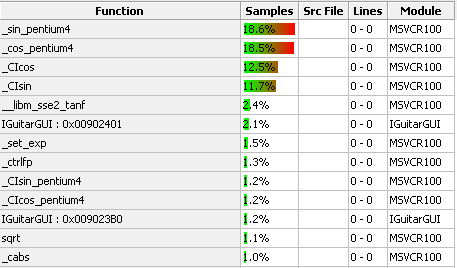
\includegraphics[width=300px]{sincos.png}
\caption{Temps passé par fonction. Données obtenues avec Luke Stackwalker, sous Windows.}
\label{player_performance}
\end{center}
\end{figure}

Les fonctions sin et cos sont en fait issues du simple calcul $e^{ix} = cos(x) + i*sin(x)$.
Elles sont disponibles sous plusieurs formes car les optimisations du compilateur (\ac{MSVC} ici) ont été activées dans leur niveau maximal (avec l'option \texttt{-O2}).

Or, après étude du code, il est apparu que les exponentielles calculées ont toujours des paramètres connus :
\begin{figure}[H]
\begin{lstlisting}
x = (double) ((i%d)*(n/(2*d)));
w = cexp(-I*(2*M_PI*x) / n );
\end{lstlisting}
\caption{Calcul d'exponentielle complexe, extrait de \texttt{fft.c : butterfly}}
\label{api_cexp}
\end{figure}

Ici, i, d et n sont des entiers. Une manière possible d'améliorer de manière drastique les performances serait donc d'effectuer
un pré-calcul de ces facteurs, et de les mettre dans un dictionnaire qui serait appelé par la suite.

Ceci dit, pour améliorer temporairement les performances, nous avons tenté d'utiliser OpenMP dans la dernière boucle qui calcule
les coefficients de la fonction butterfly, ce qui permet d'utiliser les capacités des processeurs multicoeurs si l'ordinateur cible en dispose. Néanmoins, cela ne fonctionne que sous Linux avec \ac{GCC} et Windows avec \ac{MSVC}, mais pas sous Mac OS X avec Clang. Nous avons donc commenté la ligne de code qui y correspondait.

\subsection{Chronologie de l'architecture de notre logiciel}

\scalebox{1}{
\begin{tabular}{r |@{\hspace{-2.3pt}$\bullet$ \hspace{5pt}} l}

Début du projet & Editeur et lecteur séparés, pas d'\ac{API}, pas multiplateforme.\\
Fin Novembre & Création de l'\ac{API}, ajout de FMOD dans l'\ac{API} pour l'éditeur. \\
Mi-Décembre & Portage Windows, ajout de BOOST. L'éditeur utilise l'\ac{API} et exporte en XML.\\
Début Janvier & Portage Mac OS X. Début de la conception de l'interface du lecteur.\\
Début Février & Passage à Qt5, suppression de BOOST.\\
Mi-Février & Compilation native sous Windows.\\
Fin Février & Suppression de IScoreLight et création d'un nouveau manager pour le lecteur.\\
Début Mars & Le lecteur utilise entièrement l'\ac{API}.\\
Mi-Mars & Suppression de libsndfile, avantageusement remplacé par FMOD dans le lecteur.\\
Fin Mars & Utilisation de Clang sur Mac OS X, \ac{MSVC} sur Windows.\\

\end{tabular}
}

\section{Problèmes rencontrés, problèmes résolus}

Le développement de GuitarTutor ne s'est pas fait sans heurts. Nous sommes néanmoins parvenus à résoudre les différents problèmes auxquels nous avons été confrontés au cours des phases de développement.

\subsection{Reprise de code}

Comme c'était prévu, la reprise du code existant fut notre première grande étape de développement. Passé le moment de découragement lié à l'absence total de commentaires et de documentation dans la grande majorité du code source qui nous intéressait, nous nous sommes attelés à ``débroussailler'' le dépôt en mettant en place une documentation, en commentant le code, ainsi qu'en supprimant purement et simplement les portions inutilisées, qui représentaient tout de même une quantité de code loin d'être négligeable (parfois de simples fonctions, parfois des fichiers, et parfois des dossiers entiers\dots).

Par ailleurs, du fait que le projet ait été constitué de plusieurs blocs de code émanant de différentes équipes de développeurs, nous avons pu remarquer que les conventions de codage n'avaient pas été harmonisées. Nous avons pris soin de réparer cette erreur afin de faciliter la relecture et donc la réutilisation de ce même code. Les outils de refactorisation de Qt, bien qu'imparfaits, nous ont été particulièrement
utiles, en permettant par exemple la transformation d'un nom de variable en camelCase, répercuté sur toutes ses utilisations.

Passés ces quelques semaines de nettoyage et d'assimilation du code existant, nous avons pu commencer à apporter les modifications établies dans le cahier des charges, bien que, tout au long du développement, nous ayons continué la refactorisation (par exemple les suppressions de certaines bibliothèques, évoquées plus loin dans ce rapport).

\subsection{Refonte de l'interface du lecteur}

La refonte totale de l'interface du lecteur s'est présentée comme un véritable défi. Il s'agissait en effet de supprimer tout ce qui concernait l'interface dans le projet existant, et d'y mettre à la place notre propre code. Évidemment, il n'était pas question de se limiter à une structure identique à l'interface existante, celle-ci étant véritablement limitée en terme de fonctionnalités, voire clairement repoussante pour un jeune guitariste débutant. Fort heureusement, le lecteur était déjà plut\^ot bien décomposé selon le modèle MVC, ce qui nous a tout de m\^eme motivés à tenter l'expérience.

La nouvelle interface a donc initialement été développée seule, totalement séparée du reste du projet, en utilisant des faussaires pour simuler une grille d'accords, et ce selon une maquette que nous avions soumise à nos clients (voir figure \ref{annexe_proto_player} en annexe). Ce n'est qu'au bout de plusieurs semaines de développement que nous avons enfin pu intégrer la nouvelle interface au reste du projet. Cette intégration ne s'est pas faite sans heurts, mais a finalement aboutie, comme nous l'espérions (voir figure \ref{interface_player}).

\begin{figure}[H]
\begin{center}
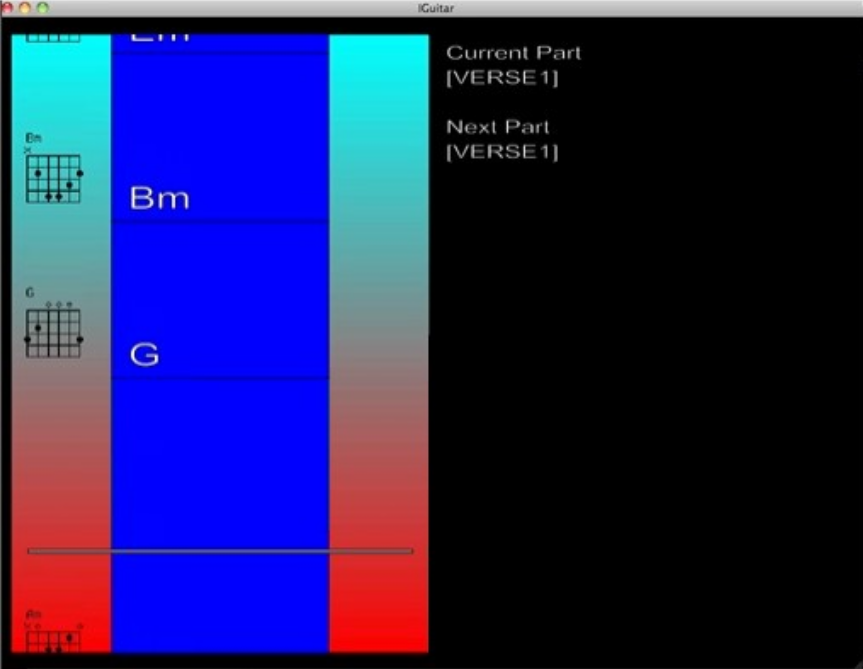
\includegraphics[width=175px]{ancien_player.png}
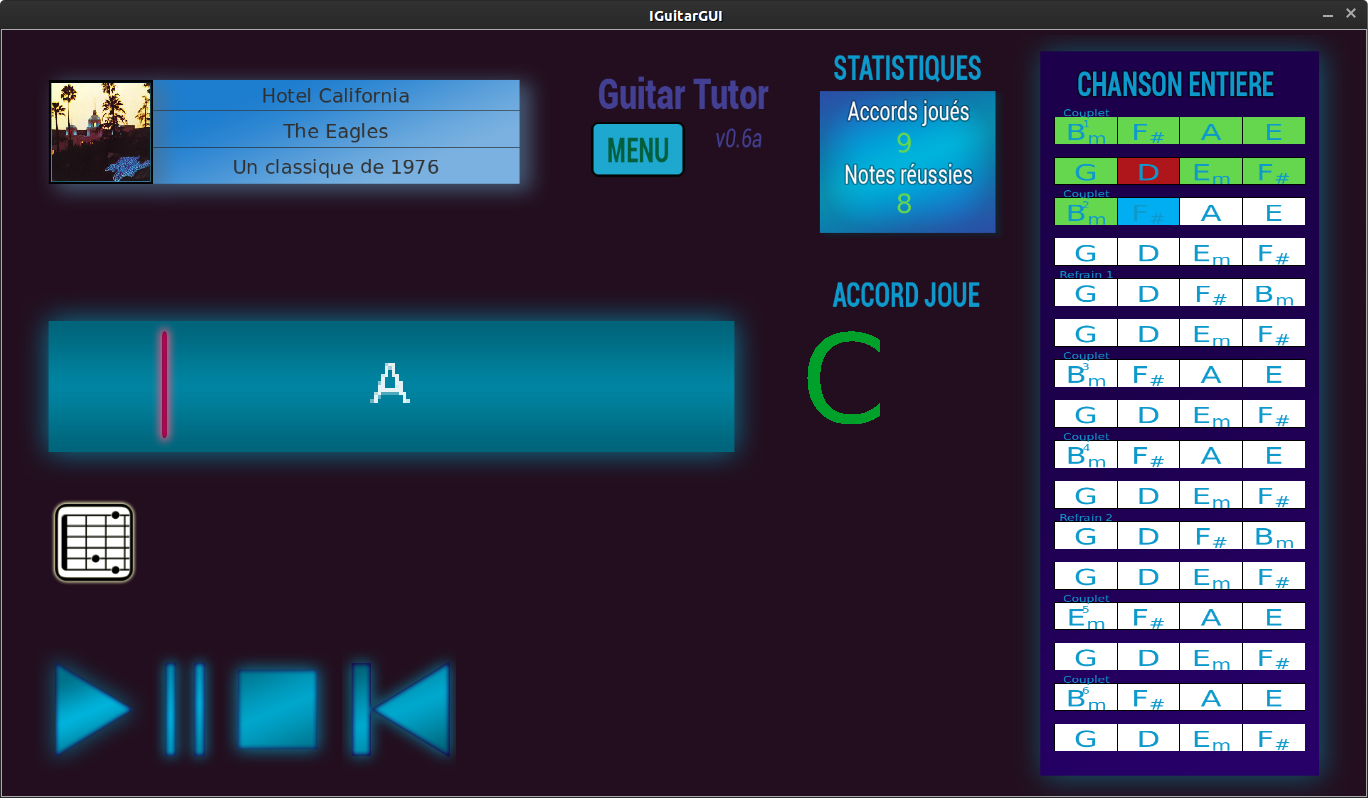
\includegraphics[width=275px]{interface_player.png}
\caption{L'interface du lecteur a été entièrement refaite}
\label{interface_player}
\end{center}
\end{figure}

\subsection{Portabilité}

La portabilité du logiciel, notamment sur Mac OS et Windows, faisait partie des principales demandes des clients. Les librairies utilisées jusque là était censées fonctionner à la fois sur Mac OS, Windows et GNU/Linux, et c'était une bonne raison pour ne pas en changer.

Nous nous sommes cependant rapidement rendus à l'évidence: on ne développe pas un logiciel portable simplement en utilisant des librairies portables.

\subsubsection*{Sur Mac OS}

Personne, dans notre équipe, n'ayant une machine sous Mac OS, nous avons dû nous contenter d'une version de Mountain Lion en machine virtuelle. Outre un problème d'extrême lenteur lors de la compilation et divers autres soucis liés à la connexion internet et la reconnaissance des ports USB, il était impossible de vérifier le bon fonctionnement du lecteur, puisque l'entrée audio de la VM n'était pas activée. Nous avons donc pendant longtemps développé \textit{``à l'aveugle''} sous Mac OS, où tout ce que nous pouvions faire était de vérifier que la compilation se faisait correctement.
Un temps d'adaptation a d'ailleurs été nécessaire car bien que la base du système repose sur Unix, l'ergonomie du système est très différente
de ce dont nous avons l'habitude.

Fort heureusement, un test sur une vraie machine Mac début mars nous a confirmé que le projet était bien compatible, et nous en avons également profité pour vérifier le fonctionnement de notre installateur.

Nous avons néanmoins connu des sueurs froides lors de l'intégration de la bibliothèque FMOD qui a pendant un temps causé des
problèmes sur les machines Mac réelles, alors que tout fonctionnait sous nos machines virtuelles. Cela a été l'occasion de découvrir
le système de paquetage utilisé sous Mac, ainsi que les outils qui permettent de s'en servir, comme \texttt{macdeployqt} et \texttt{install\_name\_tool}.

Enfin, s'est posé le problème du choix du compilateur. Il y a deux compilateurs principaux sous Mac : GCC et Clang.
Néanmoins, le premier n'est plus réellement supporté par Apple : la version fournie par les outils de développement Apple est la 4.2,
alors que nous en sommes à la 4.7. Clang, en contrepartie, est issu du projet LLVM et est fortement soutenu par Apple.
Bien qu'il n'offre à ce jour pas toutes les fonctionnalités de GCC (comme le support d'OpenMP, par exempl), il permet une
compilation très rapide et des performances parfois plus élevées que la dernière version de GCC (et sensiblement plus élevées que la 4.2).
Nous avons donc décidé de retenir ce dernier pour les livrables.
\subsubsection*{Sur Windows}

Le portage sous Windows a été périlleux, car le système de base n'a rien à voir avec les systèmes ayant pour base Unix et respectant
les normes POSIX que sont Linux et Mac OS X.

Notre premier réflexe a été d'utiliser MinGW qui est livré par défaut avec Qt. Néanmoins, un problème
dans la librairie winpthreads qui était livré avec la version de MinGW qui était elle-même livrée avec Qt 4.8 nous a
forcé à passer sur la librairie BOOST C++ pour un temps. De plus, en raison de l'utilisation de certaines fonctionnalitées modernes
de GCC 4.7 sous Linux, qui n'étaient pas disponibles sous MinGW 4.2, la compilation ne marchait pas sous Windows.

Nous effectuions donc un cross-compiling depuis Linux, ce qui représentait une certaine perte de temps pour les tests,
qui pour la plupart s'effectuaient d'ailleurs sous Wine, l'environnement de simulation Windows sous Linux.

Il a de plus fallu recompiler libsndfile qui n'était pas disponible directement sous Windows.

\paragraph{Arrivée de Qt5}
De ce point de vue, l'arrivée de Qt 5 a été salvatrice pour notre projet : en effet, elle mettait à jour MinGW
avec la dernière version de gcc, la 4.7, ce qui a permis une compilation directe depuis Windows, ainsi que la suppression des
threads BOOST pour un retour aux pthreads.

Nous avons de plus travaillé sur une branche qui permette la compilation avec MSVC, le compilateur C++ Microsoft.

Néanmoins, ce compilateur ne supporte pas le standard C99, qui est utilisé dans la librairie EHPCP pour représenter les types complexes.

Nous avons donc fait une tentative de portage en utilisant la classe C++ Complex, mais les performances étaient moindres au final,
ce qui nous a poussé à rester sous MinGW pour le rendu. Néanmoins, cela a été l'occasion d'apprendre les
bases de l'API Windows, notamment pour la gestion des threads.

\paragraph{Installation}
Une des autres particularités de Windows est qu'il n'y a pas de système de gestion de paquetage comme sous la majorité des systèmes Linux et Mac OS X.
Il est donc nécessaire de créer nous-même un installeur, nous avons pour ce faire utilisé Advance Installer dans sa version gratuite.

Ce logiciel permet un déploiement facile : création d'icônes dans le menu démarrer, sur le bureau, gestion des mises à jour...

\paragraph{Portaudio et performance audio basse-latence}
Contrairement à Linux et Mac OS X, dont les couches audio ALSA (pour Linux) et CoreAudio (pour Mac OS X) permettent immédiatement
des basses latences, ce n'est pas le cas sous Windows.

Cela pose problème pour le jeu de guitare : en effet, la latence de base du mixeur Windows est d'environ 40 millisecondes.
Et des mesures ont montré que l'oreille humaine arrivait à percevoir un décalage à partir de 10 millisecondes, et que cela devenait gênant pour le jeu à partir de 20 millisecondes.

Une solution a été développée par Steinberg (l'éditeur du séquenceur Cubase) : le protocole ASIO.

Ce protocole permet d'atteindre de très basses latences (parfois jusqu'à moins d'une milliseconde) avec
du matériel professionnel et de basses latences avec ASIO4ALL, un logiciel qui permet d'utiliser des cartes son standard de PC avec le protocole ASIO.

Le problème pour l'incorporation de cette technologie dans le projet est qu'il est nécessaire de compiler PortAudio avec le SDK ASIO, ce qui
ne peut se faire qu'avec MSVC, le compilateur Microsoft.
Comme l'algorithme de name-mangling de MSVC est incompatible avec celui de MinGW / GCC, il est nécessaire de recompiler tout le projet avec MSVC, ce qui cause la perte de performance vue plus haut.
De plus, il faut remplacer la DLL portaudio fournie dans le livrable avec la DLL compilée avec le support ASIO, ce qui fait
que le logiciel ne pourra pas s'exécuter sur un ordinateur sans ASIO4ALL ou une carte son professionnelle fournissant un pilote ASIO.

\subsubsection*{Sur GNU/Linux}

Il s'agit du seul des trois systèmes d'exploitation pour lequel nous n'avons pas eu de problème particulier, mais aussi le seul qui n'était pas demandé. Peut-être est-ce simplement parce que nous avons tous commencé à coder directement sur celui-ci, et que c'est aussi le système sur lequel le groupe de PFA précédent s'était focalisé.

\subsubsection*{De l'avantage de l'utilisation de multiples compilateurs}

Bien qu'à priori, on puisse penser que c'est un calvaire de maintenir un même programme fonctionnel sur plusieurs systèmes et plusieurs compilateurs, nous nous sommes rendu comptes que cela avait aussi un avantage majeur : la détection d'erreurs et d'incorrections.
Ainsi, GCC est parfois assez laxiste quand à son interprétation des standards du C++ et permet des choses qui ne sont pas toujours acceptées par les autres compilateurs.

L'utilisation de Clang et de MSVC a donc permis de soulever des approximations qui étaient passées inaperçues sous GCC mais qui contribuaient à avoir un code moins lisible.
De plus, cela nous a permis de comprendre de quelle manière l'interprétation des standards pouvait différer d'un compilateur à l'autre.

Enfin, nous avons pu mesurer des différences de performance : par exemple, sous Windows, aussi étrange que cela puisse paraître, l'exécution du lecteur nous a semblé beaucoup plus fluide lorsque compilé avec MinGW plutôt qu'avec MSVC qui est pourtant le compilateur Microsoft. Toutes les optimisations possibles étaient activées dans les deux cas.

\section{Discussion sur les choix opérés}

Du début jusqu'à la fin du projet, nous avons dû faire des choix de conduite. Nous recenserons dans cette partie les principales questions que nous nous sommes posées sur la marche à suivre.

\subsection{Environnement logiciel}

Comme il nous avait été conseillé de faire, nous nous sommes rapidement accordés sur l'environnement logiciel à adopter.
\begin{itemize}
 \item Utilisation de QtCreator, environnement de développement C++ open-source, multi-plateformes, et régulièrement mis à jour
 \item Développement sur Linux. Le choix n'était pas évident, étant donné que ce système d'exploitation ne faisait pas partie des cibles officielles du projet. L'intérêt était en fait de ne pas favoriser le développement sur Windows, avant de nous rendre compte que certains de nos choix avaient été faits au détriment de Mac OS X, ou inversement.

 Néanmoins, dès que la compilation a été possible de manière native sur Windows, un des membres du groupe est resté dessus
 pour le développement, ce qui a permis d'empêcher que des problèmes de compatibilité ne se propagent trop longtemps.

 De même, le programme était réguilèrement construit sous Mac OS X pour vérifier que la compatibilité n'était pas brisée par une manipulation malencontreuse.
 \item Utilisation du gestionnaire de version Git, et non de Subversion. La raison est que Git est de plus en plus utilisé, au détriment de SVN, et que le PFA était une excellente occasion pour apprendre à l'utiliser.
 \item Création du dépôt sur GitHub. Nous avons éliminé le dépôt de l'ENSEIRB-MATMECA en raison d'une coupure qui aura duré plusieurs jours en Octobre (en plus des fréquentes interruptions de ce service dont nous avions pris l'habitude au cours de l'année précédente), ainsi que de nombreux autres services tels que Sourceforge ou Google Code, car ceux-ci imposaient l'utilisation d'une licence libre (ce qui, a priori, n'est pas le cas de GuitarTutor) aux projets hébergés sur leur plate-forme, à moins de payer un abonnement mensuel. GitHub était également dans ce cas, mais une offre réservée aux étudiants nous a permis de bénéficier gratuitement d'un compte premium pour créer librement un dépôt privé, sans contrainte de licence.
\end{itemize}

Les différents choix énumérés ci-dessus ont été faits au début du projet en analysant les opinions de chacun, puis \textit{``officialisées''} en les listant sur notre wiki.


\subsection{Utilisation de Qt}

Le choix d'utiliser la librairie Qt s'est fait très rapidement, tant les avantages étaient évidents:
\begin{itemize}
 \item Le code source existant utilisait déjà Qt.
 \item Qt est utilisable aussi bien sur Mac OS X que sur Windows, ainsi que sur Linux.
 \item Le support officiel d'Android et iOS, les systèmes d'exploitation mobiles dominants sera effectif d'ici deux sous-versions de Qt,
 ce qui fait que le programme pourra être porté sans heurt sur tablette, smartphone... Il sera juste nécessaire d'ajuster les vues pour
 ces nouvelles plateformes.
 \item Le développement avec Qt est facilité par l'IDE que nous avons choisi, à savoir QtCreator.
 \item La documentation est très claire et complète.
 \item Qt est open-source et bénéficie d'une large communauté d'utilisateurs.
 \item Qt est incroyablement complet: interface graphique, XML, multimédia, socket, affichage de pages web\dots
 \item Plusieurs d'entre-nous avaient déjà des connaissances sur cette librairie.
\end{itemize}

Nous avons donc choisi d'adopter cette librairie dès les débuts du projet.

\subsection{Utilisation de FMOD}

FMOD est la librairie audio qui est utilisée aujourd'hui dans l'éditeur et dans le lecteur. Là encore, c'était cette même librairie qui servait déjà dans l'ancienne version de l'éditeur, dans la partie qui traitait les fichiers audio. En revanche, dans le lecteur, nous avons substitué la librairie \textit{libsndfile} pour FMOD.

FMOD comporte de nombreux avantages, comme par exemple la lecture de formats compressés tels que le MP3, aujourd'hui incontournable, mais aussi bien d'autres formats propriétaires courants, comme le WMA'.
Jusqu'à présent, \textit{libsndfile} limitait l'utilisation de GuitarTutor aux fichiers wav, ce qui contraignait l'utilisateur à manipuler des fichiers de très grande taille dans des formats non-compressés ou bien relevant de l'antiquité informatique comme Amiga, Atari\dots FMOD disposait également des mêmes fonctionnalités que celles qui étaient alors utilisées dans le code avec \textit{libsndfile}, ce qui permettait de ne pas géner la transition. FMOD nous a donc semblé être un bon choix, malgré le fait qu'il s'agisse d'une librairie propriétaire (nous n'avons pas eu de contre-indication de la part des clients à ce propos).
De plus, c'est un standard dans le monde des jeux vidéos, ce qui est une bonne formation pour ceux d'entre nous souhaitant partir dans ce domaine.


\subsection{Format d'échange en XML}
\label{xml}

L'échange entre l'éditeur et le lecteur se fait par l'intermédiaire de fichiers. Ces fichiers sont créés et modifiés par l'éditeur, puis lus dans le lecteur. Initialement, le format qui était utilisé listait les différentes parties du morceau, ainsi que les accords devant être joués et le temps en millisecondes correspondant (par rapport au début de la musique). Le fichier audio lu simultanément était, quant à lui, codé en dur dans le code source. Bien qu'il eût été facile de se contenter d'intégrer le chemin du fichier audio en début de fichier, nous avons préféré repenser totalement le format du fichier d'échange en nous basant sur le langage XML.

\begin{table}[H]
\begin{center}
\begin{tabular}{l|l}
 & \verb{<?xml version="1.0"?>{\\
 & \verb{<morceau timeSignature="4" line="16" chordMesure="1" end="261735"{ \\
 & \verb{  nom="Hotel California" comment="Un classique de 1976" column="4"{ \\
 & \verb{  fichier="Tracks/HotelCalifornia/EaglesHotelCalifornia.mp3"{ \\
 & \verb{  beginning="53145" bar="56402" artiste="The Eagles">{ \\
\verb{[COUPLET1]{ & \verb{  <partie nom="Couplet 1">{ \\
\verb{Bm 53145{ & \verb{    <accord nom="Bm" temps="53145" repetition="1"/>{ \\
\verb{F# 56402{ & \verb{    <accord nom="F#" temps="56402" repetition="1"/>{ \\
\verb{...{ & \verb{    ...{\\
 & \verb{  </partie>{\\
 & \verb{</morceau>{\\
\end{tabular}
\caption{Comparaison entre ancien et nouveau formats d'échange}
\label{fichiers_xml}
\end{center}
\end{table}

Nous avons demandé à M. Lombard, chargé de TD de XML et consultant pour Sopra Group, de nous conseiller sur la manière dont structurer notre document, et la proposition que nous lui avons faite (le format ci-dessus) lui a semblé cohérente par rapport à notre utilisation.

Comme on peut le voir sur l'exemple du tableau \ref{fichiers_xml}, notre format de fichier nous permet de contenir bien plus d'informations que l'ancien format. C'est un très gros avantage lorsqu'il s'agit notamment de recharger le fichier dans l'éditeur pour le modifier, puisque toutes les données qui ont été entrées lors de la création du fichier y ont été sauvegardées (même si certaines ne sont pas directement utilisées dans le lecteur).

Un second avantage est la facilité d'adaptation du format. En effet, si un jour il est décidé d'ajouter une nouvelle information dans le fichier XML, il n'y aura a priori pas besoin de modifier la façon de récupérer les informations. Cette maléabilité permise par le standard DOM (\textit{Document Object Model}) qui permet de naviguer au sein d'un document XML sans avoir à connaître tout son contenu. C'est justement la technique qui est mise en \oe uvre dans le module QtXML que nous avons utilisé (voir l'exemple de la figure \ref{xml_dom}).

\begin{figure}[H]
\begin{lstlisting}
//Récupération du premier accord de la partie courante
QDomNode chordNode = partElement.firstChild();
while(!chordNode.isNull())
{
  QDomElement chordElement = chordNode.toElement();

  //Récupération des informations de l'accord
  QString name = chordElement.attribute("nom", 0);
  int t = (chordElement.attribute("temps", 0)).toInt();
  int rep = (chordElement.attribute("repetition", 0)).toInt();

  //Création de l'objet représentant l'accord
  currentChord = new TrackChord(name, t, rep, previousChord, 0, currentPartTrack);
  //Ajout de cet accord à la liste des accords de la partie courante
  currentPartTrack->AddChord(currentChord);

  //Passage à l'accord suivant
  chordNode = chordNode.nextSibling();
}
\end{lstlisting}
\caption{Lecture d'un fichier XML, extrait de \texttt{TrackLoader::convertXmlToLogicalTrack}}
\label{xml_dom}
\end{figure}

\subsection{Reprise des bases précédentes}

Même s'il était au départ tentant de faire table rase et de recommencer le projet à zéro, tant la présentation du code existant laissait à désirer, nous avons fait l'effort de le remanier et de l'appréhender afin de pouvoir le réutiliser au maximum.

\subsubsection{Sur l'éditeur}

Nous avons gardé la base de l'interface de l'éditeur, à savoir le système de grilles, ainsi que le système d'arbre des accords. Nous avons ensuite ajouté peu à peu les différents éléments qui constituent aujourd'hui l'éditeur de grilles (voir figure \ref{av_ap_editeur}).

\begin{figure}[H]
\begin{center}
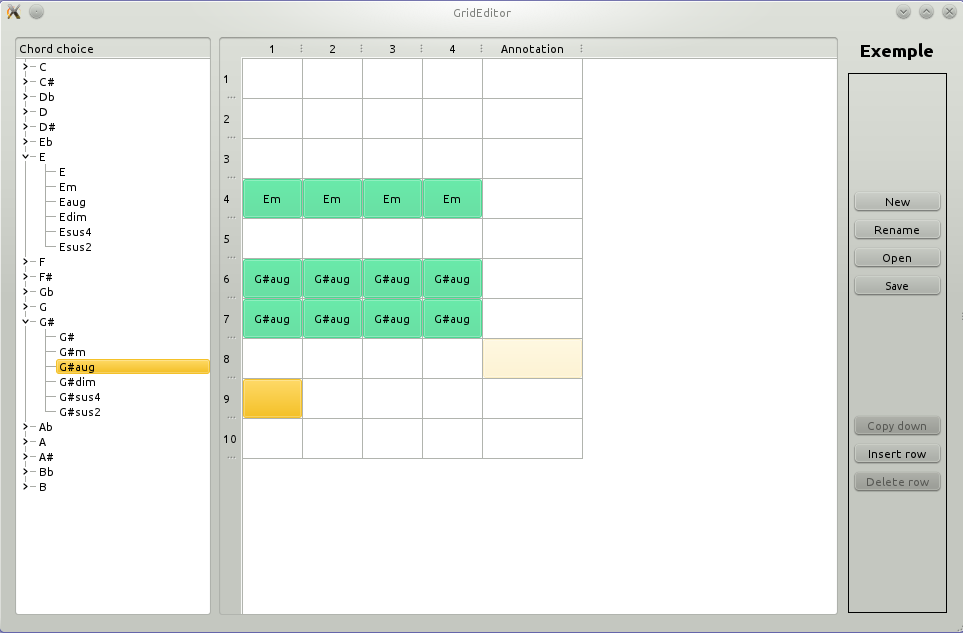
\includegraphics[width=225px]{ancien_editeur.png}
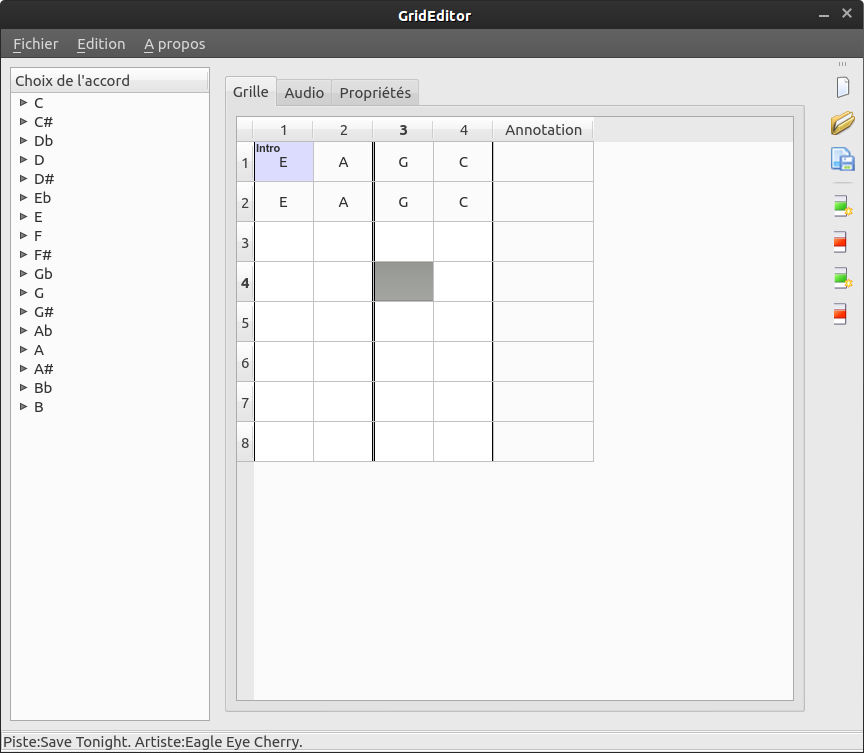
\includegraphics[width=225px]{nouveau_editeur.png}
\caption{L'éditeur de grilles, avant et après}
\label{av_ap_editeur}
\end{center}
\end{figure}


\subsubsection*{Quelques mots sur l'interface}

Un des points importants qui étaient à prendre en compte lors du développement était la nécessité de réaliser un logiciel accessible. L'expérience utilisateur était par conséquent un des facteurs clés. Le problème était que la tâche que l'utilisateur final doit réaliser avec le logiciel demandait un savoir-faire particulier (par exemple, synchroniser un tableau avec un morceau de musique), et il était donc primordial de la rendre le plus accessible possible, sans pour autant limiter les fonctionnalités.

Nous avons fait le choix de penser en premier lieu à l'expérience utilisateur, en créant une interface qui soit à la fois accessible et esthétique. Nous avons par exemple apporté:
\begin{itemize}
 \item la traduction en Français de l'interface
 \item la possibilité d'ajouter les accords au clavier, comme il serait tentant de faire, ainsi que le déplacement par tabulations
 \item une meilleure visibilité du découpage en mesures et en parties de la grille, et la possibilité de rentrer plusieurs accords par mesure
 \item une barre d'outils pour les actions les plus fréquentes, ainsi que des raccourcis claviers
 \item le rapprochement implicite entre la grille et le morceau (système d'onglets, et fusion des deux anciens éditeurs en un seul)
 \item la visualisation de l'information contenue dans le fichier audio
\end{itemize}

Le principal défi aura été de faciliter la synchronisation entre le morceau et la grille. Nous avons dans un premier temps mis en place un lecteur audio au sein de l'éditeur afin que l'utilisateur puisse aisément écouter le morceau qu'il est en train de créer. C'est ensuite qu'est venue l'idée, notamment à l'aide de nos clients, d'utiliser trois marqueurs temporels pour définir cette synchronisation:
\begin{enumerate}
 \item Un marqueur pour le début de la première mesure du morceau
 \item Un second marqueur pour signaler la fin de la première mesure
 \item Et un dernier pour signaler la fin du dernier accord du morceau
\end{enumerate}
Une fois les temps associés définis précisément, il est facile de définir le temps de début de chaque accord dans le morceau (voir l'algorithme sur la figure \ref{editor_time_caseitems}). Cette méthode nous a semblé particulièrement adaptée à notre situation, puisque les morceaux ciblés par l'application sont des morceaux qui sont rythmiquement très stables (c'est-à-dire que la durée de chaque mesure est supposée constante). De cette façon, l'utilisateur ne doit que très peu intervenir en comparaison avec l'ancienne méthode qui consistait à lui faire taper chaque temps du morceau.

Néanmoins, si nécessaire, l'utilisateur peut ajuster le temps mesure par mesure, et peut propager le changement sur une mesure à toutes
les mesures suivantes, comme dans le cas ou on rajouterai deux temps de pause entre un refrain et un couplet par exemple.

\begin{figure}[H]
\begin{lstlisting}
for (int r = 0 ; r < rmax ; r++) //Parcours des lignes
{
	for (int c = 0 ; c < cmax - 1 ; c ++) //Parcours des colonnes
	{
		QTime caseTime = MsecToTime(
				    (TimeToMsec(beginning) +
				      ((TimeToMsec(bar) - TimeToMsec(beginning))
				        /m_barsize)
				    * (r * (cmax - 1) + c)));
		((CaseItem*) item(r,c))->setBeginning(caseTime);
	}
}
\end{lstlisting}
\caption{Mise en place des temps de début des accords en fonction des marqueurs entrés par l'utilisateur, extrait de \texttt{ChordTableWidget::setTimeInfo}}
\label{editor_time_caseitems}
\end{figure}

La question était donc de trouver un moyen simple pour pouvoir indiquer de façon précise chacun de ces trois marqueurs temporels. Il nous est tout de suite venu à l'esprit d'utiliser les formes d'ondes du fichier audio désiré pour mieux cibler les débuts des accords. FMOD, pour les données spectrales, et Qt, pour l'interface, ont été très utiles pour l'implémentation. Un zoom et déplacement à la souris, inspiré de l'ergonomie des \ac{DAW} actuels, a également été mis en place sur cette même forme d'onde, ainsi que le positionnement des timers directement \textit{sur} la forme d'onde. Au final, le marquage devient une tâche relativement aisée et rapide (figure \ref{editor_audiosync}).

Enfin, dans le cas idéal ou le morceau aurait été joué au métronome, on peut directement rentrer le tempo dans l'éditeur.
\begin{figure}[H]
\begin{center}
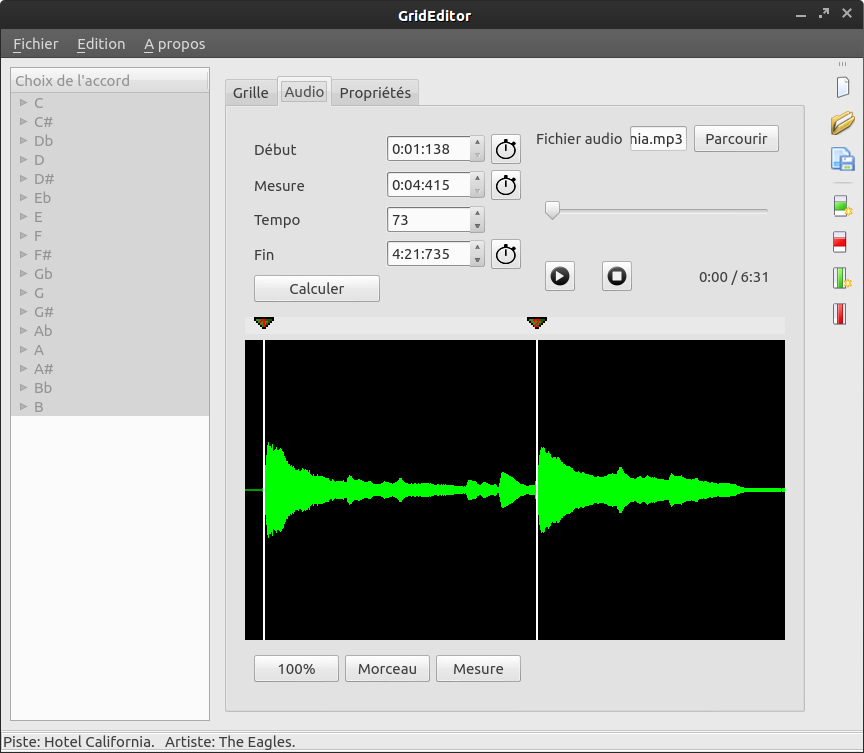
\includegraphics[width=400px]{editor_audiosync}
\caption{Synchronisation audio}
\label{editor_audiosync}
\end{center}
\end{figure}

\subsubsection{Sur le lecteur}

En ce qui concerne le lecteur, nous n'avons dans un premier temps que modifié l'interface. Celle-ci a été refaite intégralement selon la maquette qui avait été présentée en janvier (voir la figure \ref{annexe_proto_player} en annexe). Notre travail a finalement abouti à une interface semblable aux exigences qui avaient été fixées, certains détails ayant été revus en cours de développement en accord avec nos clients. L'objectif principal était de rendre le programme beaucoup plus convivial, mais aussi plus accessible. L'interface actuelle est présentée en figure \ref{interface_player}.

Dans un deuxième temps, nous avons fait le choix de revoir le fonctionnement interne du lecteur. Comme évoqué précédemment, nous avons ainsi commencé par faire disparaître la librairie \textit{IScoreLight}. En effet, celle-ci comportait plusieurs dizaines de fichiers sources (en pratique, 17000 lignes de code) qui, au final, n'étaient pas exploitées. De plus, le format que nous avons défini dans les classes \texttt{LogicalTrack}, \texttt{PartTrack} et \texttt{TrackChord} remplit exactement le besoin de positionnement dans le morceau que nous avions défini. La gestion de la navigation dans le morceau est donc confiée à la classe \texttt{SongManager} que nous avons créée.

Dans un deuxième temps, nous nous sommes attelés à remplacer la librairie \textit{libsndfile} par FMOD en vue de supporter de nouveaux formats audio. FMOD se charge en fait d'ouvrir le fichier audio demandé et de le mettre en mémoire. La gestion à proprement parler du son reste la tâche de PortAudio dans le lecteur.

Nous ne l'avons pas fait par manque de temps, mais l'idéal serait de remplacer aussi PortAudio par FMOD,
 ce qui peut se faire sans trop de problèmes car FMOD gère aussi les entrées audio.
 Cela permettrait de partager le code de lecture entre le lecteur et l'éditeur, ce qui n'est pas le cas actuellement.
 De plus, comme vu précédemment avec PortAudio, FMOD permet aussi de gérer les cartes sons ASIO, ce qui permettrait de basses
 latences pour l'entrée sous Windows.

Finalement, il ne reste aujourd'hui de la première version du lecteur que la gestion bas niveau du son, notamment l'analyse des accords effectuée par la librairie \textit{EHPCP}. Ce tri nous a permis d'améliorer grandement les performances, notamment lors de la compilation du programme (cf. figure \ref{refonte_code}).

\begin{figure}[H]
\begin{center}
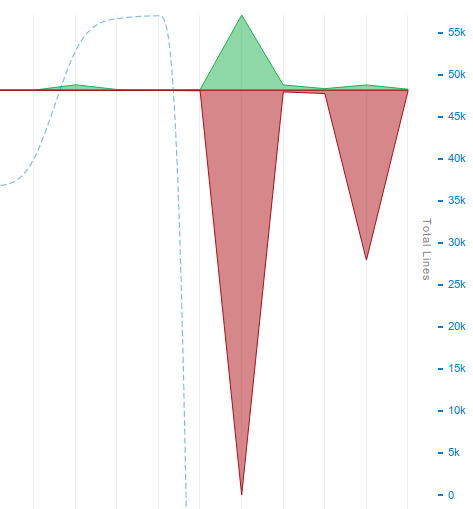
\includegraphics[width=300px]{refonte_code.png}
\caption{Suppression des bibliothèques Boost et IScoreLight du projet}
\label{refonte_code}
\end{center}
\end{figure}

Nous avons également fait en sorte que le lecteur utilise par défaut OpenGL, afin que celui-ci soit, au moins partiellement, exécuté sur la carte graphique de l'utilisateur, en vue d'améliorer là encore les performances. En effet, nous n'utilisons pas le système de widgets standard comme sur l'éditeur par exemple: nous avons utilisé le système de scène de Qt, qui permet plus de liberté graphique, ce que nous pensons adapté au monde ludique.
Ce système de scène est tout à fait représentatif de la \ac{MVC} : nous plaçons les éléments comme nous le désirons et Qt se charge
de la logique de mise à jour, de dessin, et de boucle centrale. Il suffit donc simplement de dire à Qt d'utiliser OpenGL via la ligne suivante :

\begin{figure}[H]
\begin{lstlisting}
setViewport(new QGLWidget);
\end{lstlisting}
\caption{Activation d'OpenGL dans le lecteur, extrait de \texttt{MyView::MyView}}
\label{player_opengl}
\end{figure}

et le dessin passe, lorsque c'est possible (c'est le cas sur tout ordinateur récent avec des pilotes graphiques à jour), par la carte graphique.

\subsection{Installateurs sur les différents systèmes d'exploitation}

Comme il nous avait été demandé, le programme devait être rendu sous la forme d'un installateur pour chacun des deux systèmes d'exploitation visés.

\subsubsection{Sur Windows}

Sur Windows, GuitarTutor se présente sous la forme d'un installateur \textit{msi} créé avec le logiciel Advance Installer. L'apparence de cet installateur est tout à fait semblable aux installateurs de logiciels Windows habituels, et propose les mêmes options; comme par exemple la possibilité de modifier le chemin de l'installation, ou encore celle de créer une icône sur le bureau de l'utilisateur.

La seule véritable difficulté sur ce système d'exploitation aura été de définir quelles étaient les librairies dynamiques à inclure dans notre package. Pour cela, nous avons testé sur des machines vierges de tout outil lié à notre environnement de travail (Qt, FMOD,\dots), puis simplement procédé par élimination pour ne retenir que les fichiers dll nécessaires.

Un outil qui a aussi été utilisé vers la fin du projet est Dependency Walker : ce programme analyse un fichier exécutable et liste les
DLL dont il a besoin.

\begin{figure}[H]
\begin{center}
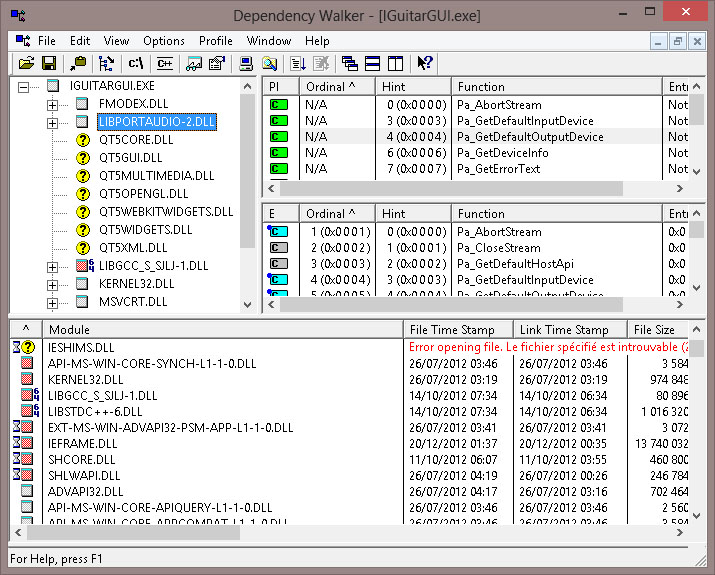
\includegraphics[width=300px]{depwalker.jpeg}
\caption{Dependency Walker}
\label{dep_walker}
\end{center}
\end{figure}

Nous avions un temps pensé à recompiler Qt de manière statique pour limiter la taille du programme ainsi que l'installation de DLL mais cela s'est révélé trop complexe à mettre en oeuvre.

\subsubsection{Sur Mac OS X}

Sur Mac OS X, notre programme se présente comme une application \textit{.app}, autrement appelé \textit{bundle}. C'est avec le format \textit{dmg}, sur ce système d'exploitation, une des deux formes les plus usuelles pour distribuer un logiciel. Il s'agit en fait d'un dossier contenant l'exécutable en lui-même, ainsi que tous les éléments tels que les bibliothèques dynamiques nécessaires à son fonctionnement (cf figure \ref{app_mac_os}).

\begin{figure}[H]
\begin{center}
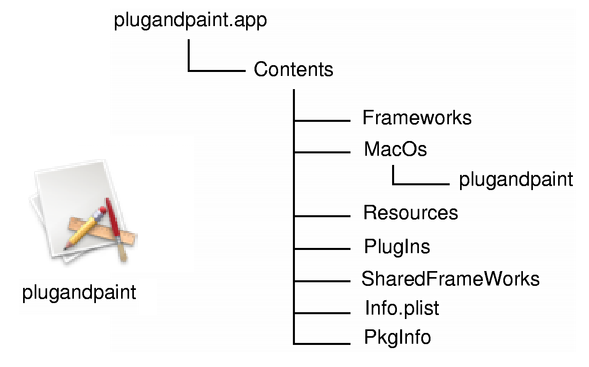
\includegraphics[width=300px]{bundle_mac.png}
\caption{Le bundle pour Mac OS X (d'après qt-project.org)}
\label{app_mac_os}
\end{center}
\end{figure}

Plusieurs outils similaires sont mis à la disposition des développeurs Mac OS X pour créer ces bundles. Nous avons, dans un premier temps, choisi d'utiliser l'utilitaire \textit{qtmacdeployment}, fourni avec Qt. Seulement, il s'est avéré que les bundles créés ne fonctionnaient pas sur toutes les machines en raison d'un problème concernant la bibliothèque dynamique de FMOD. Nous avons finalement opté pour un autre outil, du nom de \textit{install\_name\_tools}, fourni cette fois-ci avec l'environnement XCode, et qui a réglé notre problème de déploiement.

\subsection{Développement Agile}

En accord avec les conseils de notre responsable pédagogique, nous avons rapidement opté pour l'utilisation d'une méthode de développement de type agile. Le PFA état en effet une excellente occasion pour s'essayer à ce genre de méthodes qui sont de plus en plus employées dans des cadres professionnels.

\subsubsection{Réunions clients}

Dès le mois de novembre, nous avons mis en place un système de rendez-vous réguliers, généralement toutes les trois semaines avec nos clients. Ces réunions servaient tout d'abord à présenter le travail qui avait été effectué depuis le dernier rendez-vous, au travers d'une démonstration sur le logiciel en cours de développement. S'en suivait une discussion sur les différents points qui méritaient d'être relevés, afin de répartir les tâches en trois catégories: ce qui était fait et qui était validé, ce qui était fait mais restait à améliorer (ou à changer totalement), et enfin, ce qui restait à faire. Il ne restait alors qu'à fixer les objectifs à tenir d'ici le prochain rendez-vous.

Les avantages de travailler de la sorte se sont révélés au cours du projet. Tout d'abord, la possibilité de discuter de manière régulière de nos avancées avec nos clients était particulièrement intéressante, car cela permet d'instaurer un dialogue entre demandeurs et réalisateurs. On peut notamment remarquer que le cahier des charges (cf annexes) comporte plusieurs points qui n'ont pas été réalisés, ou qui ont été réalisés différemment de ce qui était initialement prévu, pas à cause d'un manque de temps, mais grâce à ce dialogue qui a permis d'affiner et de changer les besoins exprimés au fur et à mesure du développement du projet.

La figure \ref{agile} résume ce processus.

\begin{figure}[H]
\begin{center}

\includegraphics[width=450px]{methode_agile.png}
\caption{Schéma du processus de développement agile}
\label{agile}
\end{center}
\end{figure}

\subsubsection{Organisation de l'équipe et du travail}

De manière analogue au \textit{ScrumMaster} de la méthode Scrum, nous avons choisi au sein de notre équipe une personne en charge de veiller à la bonne application de notre méthode de développement. Sans se situer à un niveau supérieur aux autres, comme ce serait le cas pour un chef de projet, cette personne devait centraliser les travaux et les impressions de chacun pour aider à la répartition des tâches. Elle servait par ailleurs de \textit{représentant} de notre équipe pour nos clients et notre responsable pédagogique.

Les tâches étaient ensuite attribuées selon les demandes du cycle courant et des préférences de chacun, généralement par binômes, binômes qui ont été très variables tout au cours du projet. Des réunions hebdomadaires permettaient de faire le point sur les difficultés rencontrées et l'avancement des différentes tâches, et éventuellement de réorganiser la répartition. En plus de cela, l'équipe était informée par mail des interrogations et des avancées entre deux réunions, ainsi que par l'intermédiaire de notre wiki que nous avons mis en place dès le début du projet.

De manière générale, cette méthode de développement semble avoir bien fonctionné pour notre équipe au cours de ce projet.

\subsubsection{L'agile dans le code}
Un des autres aspects de l'approche agile au développement de projet est l'impact sur
la manière de produire du code. Notamment, comme cela a pu être vu au début du rapport dans la
chronologie du projet, il y a eu énormément de refactorisations et de changements assez profonds,
qui ont été annulés par la suite, comme pour BOOST, ou maintenus, comme pour FMOD.

\subsubsection{L'agile dans le cadre de l'école}
La difficulté principale avec le développement agile se situe dans les contraintes de temps
imposées par l'école et l'emploi du temps, dont les deux défauts sont d'être fixe (on ne peut pas ne pas aller en cours)
et variable (les horaires d'un même cours peuvent changer d'une semaine à l'autre).

De plus, notre répartition dans des groupes de TD différent a fait que nous n'avons pas toujours pu nous voir
comme nous le voulions, et que le gros du travail et des sprints était ainsi effectué généralement chez soi, en
communiquant par e-mail.

Ce qui aurait du être des post-its sur un tableau avec des tâches marquées dessus s'est retrouvé être un wiki
ou chacun pouvait barrer la tâche qu'il prenait en charge, néanmoins cette méthode est moins conviviale.

Le plus problématique dans cette approche est que la communication est plus difficile avec les autres
quand un binôme est bloqué, notamment.


\section*{Conclusion}

\subsection*{Un objectif atteint}

Nos clients avaient été très clair à ce sujet lors de la présentation du projet: l'objectif était, à la fin du PFA, de fournir deux programmes totalement fonctionnels et prêts pour une démonstration en école de musique.

Nous avons remis à nos clients, peu de temps avant la date finale des projets, une version en \textit{pre-release} de GuitarTutor afin qu'ils puissent avoir un réel aperçu du programme et que nous puissions, le cas échéant, corriger quelques détails. Ceux-ci semblent avoir été particulièrement satisfaits du travail que nous avons réalisé, et c'est là le plus important pour notre propre satisfaction. Le deuxième point est sans doute le fait que nous pensons clairement avoir atteints les objectifs qui étaient demandés. Nous avons en effet réalisé une suite logicielle qui, à notre sens, semble parfaitement utilisable dans le contexte cible - c'est-à-dire en école de musique - et c'était d'ailleurs ce vers quoi nous avons orienté notre développement. La compatibilité du projet sur les systèmes Windows et Mac est elle aussi parfaitement respectée, malgré les difficultés loin d'être négligeables auxquelles nous avons été confrontés.

En sus, la reprise de l'ancien code nous a fait comprendre l'importance de produire un code de qualité et de tout faire pour faciliter la reprise ultérieure, éventuellement par des personnes tierces. C'est pourquoi nous avons soigné notre code source en fournissant une documentation exhaustive de notre travail ainsi qu'un code propre et clair (du moins, selon nos critères). Des optimisations ont également été apportées alors qu'elles n'étaient pas explicitement demandées, telles que le nettoyage des librairies inutilisées, la gestion du format MP3, la limitation des fuites mémoires, ou encore l'utilisation d'OpenGL pour améliorer les performances.

\subsection*{Un travail d'équipe, une expérience de travail professionnel}

Le PFA aura également été l'opportunité d'apprendre à gérer un véritable travail en équipe, d'adopter une méthode de développement, ainsi que de connaître des outils comme Git ou la librairie Qt, qui, sans être incontournables, font de même bonne figure sur un CV. C'était aussi l'occasion de débattre et de rechercher des informations sur la manière d'implémenter les choses; ou encore de travailler à partir d'un code existant.

En clair, il s'agissait de savoir se comporter dans un contexte quasi-professionnel et c'est sans aucun doute une expérience extrêmement enrichissante.
%Ce que nous a apporté le projet
%Apprentissage de librairies complexes
%Si chacun veut mettre un mot personnel ici...


\chapter{Annexes}


\end{document}
